
\documentclass[letterpaper, 10 pt, conference]{ieeeconf}  % Comment this line out if you need a4paper
\IEEEoverridecommandlockouts                              % This command is only needed if 
                                                          % you want to use the \thanks command
\overrideIEEEmargins                                      % Needed to meet printer requirements.


% Bibliography
\usepackage{biblatex}
\addbibresource{references.bib}

% Math
\usepackage{physics}
\usepackage{siunitx}
\sisetup{output-exponent-marker=\ensuremath{\mathrm{e}}}
\usepackage{amsmath}
\usepackage{amsfonts}
\usepackage{amssymb}
\usepackage{gensymb}

% Optimization and Algorithms
\usepackage{optidef}
\usepackage{algorithmicx}
\usepackage{algorithm,algpseudocode}

% Formatting
\usepackage{xcolor}
\usepackage{bm}  % for bold symbols 
\usepackage{booktabs}  % better tables
\usepackage{pifont}  % for x mark
\usepackage{graphicx}
\usepackage{hyperref}

% Plotting
\usepackage{pgfplots}
\pgfplotsset{compat=1.15,
	legend style={font=\footnotesize},
}
\usepackage{tikzscale}
% \pgfplotsset{every axis plot post/.style={
%     very thick,
% }
% }

% Custom commands
\newcommand{\half}{\frac{1}{2}}
\newcommand{\R}{\mathbb{R}}
\newcommand{\Q}{\mathbb{S}^3}
\newcommand{\skewmat}[1]{[#1]^\times}

\newcommand{\rmap}{\varphi}
\newcommand{\invrmap}{\varphi^{-1}}

\newcommand{\dR}{\delta \mathcal{R}}
\newcommand{\rot}{ \mathcal{R} }
\newcommand{\dq}{\delta q}
\newcommand{\q}{\textbf{q}}
\newcommand{\eq}{_\text{eq}}
\newcommand{\traj}[2][N]{#2_{0:{#1}}}
\newcommand{\pass}{{\color{green} \checkmark}}
\newcommand{\fail}{{\color{red} \ding{55}}}

\newcommand{\todo}[1]{\textcolor{red}{TODO: #1}}


\title{\LARGE \bf
Planning with Attitude
}

\author{Brian Jackson$^1$, Kevin Tracy$^1$, and Zachary Manchester$^1$%
    \thanks{
        $^1$Robotics Institute, 
        Carnegie Mellon University, 
        5000 Forbes Ave, Pittsburgh, PA, USA
    }
}

\begin{document}
\maketitle

\begin{abstract}
Planning trajectories for floating-base robotic systems that experience
large attitude changes is challenging due to the nontrivial group structure of 3D
rotations. This paper introduces a powerful and accessible approach for 
optimization-based planning on the space of rotations based on vector calculus and
linear algebra. We demonstrate the effectiveness of the approach by adapting Newton's
method to solve the canonical Wahba's problem, and modifying the ALTRO solver for 
constrained nonlinear trajectory optimization to plan directly on the space of unit 
quaternions, achieving superior convergence on problems involving significant changes 
in attitude.
\keywords{motion planning and control, quaternions, optimal control, 
linear quadratic regulator
}
\end{abstract}

\section{INTRODUCTION}

    Many useful robotic systems---including quadrotors, airplanes, satellites, autonomous
    underwater vehicles, and quadrupeds---can perform arbitrarily large three-dimensional
    translations and rotations as part of their normal operation. While representing
    translations is straightforward and intuitive, effectively representing the
    nontrivial group structure of 3D rotations has been a topic of study for many
    decades. Although we can intuitively deduce that rotations are three-dimensional, a
    globally non-singular three-parameter representation of the space of rotations does
    not exist \cite{stuelpnagel1964parametrization}. As a result, when parameterizing
    rotations, we must either a) pick a three-parameter representation and deal with
    discontinuities, or b) pick a higher-dimensional representation and deal with
    constraints between the parameters. While simply representing attitude is nontrivial,
    generating and tracking motion plans for floating-base systems is an even more
    challenging problem.

    Early work on control problems involving the rotation group dates back to the 1970s,
    with extensions of linear control theory to spheres \cite{Brockett1973} and $SO(3)$
    \cite{Baillieul1978}. Effective attitude tracking controllers have been developed for
    satellites \cite{wie1985quaternion}, quadrotors
    \cite{Fresk2013,Liu2015,lee2010geometric,
    Johnson2005,watterson2020control,mellinger2011minimum}, and a 3D inverted pendulum
    \cite{Chaturvedi2009} using various methods for calculating three-parameter attitude
    errors.

    More recently, these ideas have been extended to trajectory generation
    \cite{Zefran1998}, sample-based motion planning \cite{Zefran1999,Kuffner2004}, and
    optimal control. Approaches to optimal control on attitude problems include
    analytical methods applied to satellites \cite{Spindler1998}, discrete mechanics
    \cite{Kobilarov2011,Kobilarov2014, Lee2008}, a combination of sampling-based planning
    and constrained trajectory optimization for satellite formations \cite{Garcia2005,
    Aoude2008}, projection operators \cite{Saccon2013}, or more general theory for
    optimization on manifolds \cites{watterson2018trajectory}. Nearly all of these
    methods rely heavily on principles from differential geometry and Lie group theory;
    however, despite these works, many recent papers in the robotics community continue
    to apply traditional methods for motion planning and control with no regard for the
    group structure of rigid body motion \cite{Alothman2016,deCrousaz2015,
    Williams2017,Geisert2016}.
    
    In this paper, we make a departure from previous approaches to geometric planning and 
    control that rely heavily on ideas and notation from differential geometry, 
    and instead use only basic mathematical tools from linear algebra and calculus that 
    should be familiar to most roboticists. 
    Similar to \cite{Mandic2011,Xu2016}, in Sec. \ref{sec:Quaternion_Calculus} we introduce 
    a quaternion differential calculus, but take a significantly simpler and more general 
    approach, enabling straight-forward adaptation of 
    existing algorithms to systems with quaternion states. 
    To make this concrete, in Sec. \ref{sec:Wahbas} we apply this method to the canonical
    Wahba's problem and demonstrate dramatically superior convergence to approaches that
    fail to properly account for the group structure. 
    In Sec. \ref{sec:trajopt} we extend these ideas to the problem of trajectory optimization,
    and detail modifications to ALTRO, a state-of-the-art constrained trajectory optimization
    solver, and demonstrate the performance gains on several constrained benchmark problems.
    To our knowledge, there does not currently exist a solver that is capable of leveraging
    the unique Markovian structure of the fixed-horizon trajectory optimization problem while
    correctly accounting for the group structure of 3D rotations.
    In summary, our contributions include:

    \begin{itemize}
        \item A unified approach to quaternion differential calculus entirely based on
        standard vector calculus and linear algebraic operations, and
        \item a fast and efficient solver for trajectory optimization problems with 
        attitude dynamics and nonlinear constraints that correctly accounts for the group
        structure of 3D rotations during the solve.
    \end{itemize}


\section{Background}

    We begin by defining some useful conventions and notation. 
    Attitude is defined as the rotation from the robot's body frame to a global inertial 
        frame. 
    We also define gradients to be row vectors, that is, for 
        $f(x) : \R^n \to \R$, $\pdv{f}{x} \in \R^{1\times n}$.

    \subsection{Unit Quaternions} \label{sec:quaternions}
        We leverage the fact that quaternions are linear operators and that the space of 
        quaternions $\mathbb{H}$ is isomorphic to $\R^4$ to explicitly 
        represent---following the Hamilton convention---a quaternion $\q \in \mathbb{H}$ as 
        a standard vector $q \in \R^4 := [q_s \;\; q_v^T]^T$ where $q_s \in \R$ and 
        $q_v \in \R^3$ are the scalar and vector part of the quaternion, respectively.
        
        Quaternion multiplication is defined as
        \begin{equation} \label{eq:quat_mult}
            \q_2 \otimes \q_1 = L(q_2) q_1 = R(q_1) q_2
        \end{equation}
        where $L(q)$ and $R(q)$ are orthonormal matrices defined as
        \begin{align}
            L(q) &:= \begin{bmatrix} 
                q_s \;\; & -q_v^T \\ 
                q_v \;\; & q_s I + \skewmat{q_v} 
            \end{bmatrix} 
            \label{eq:Lmult} \\
            %= \begin{bmatrix} q & G(q) \end{bmatrix} \label{eq:Lmult} \\
            R(q) &:=\begin{bmatrix} 
                q_s \;\; & -q_v^T \\ 
                q_v \;\; & q_s I - \skewmat{q_v} 
            \end{bmatrix} \label{eq:Rmult},
        \end{align}
        and $\skewmat{x}$ is the skew-symmetric matrix operator
        \begin{equation}
            \skewmat{x} := \begin{bmatrix} 
                0 & -x_3 & x_2 \\ 
                x_3 & 0 & -x_1\\ 
                -x_2 & x_1 & 0 
            \end{bmatrix}.
        \end{equation}
        
        The inverse of a unit quaternion $q^{-1}$, giving the opposite rotation, is equal 
        to its conjugate $q^*$, which is simply the same quaternion with a negated vector 
        part:
        \begin{equation} \label{eq:T}
            \q^* = T q := \begin{bmatrix} 
                1 & \\ 
                & -I_3 
            \end{bmatrix} q
        \end{equation}
        The following identities, which are easily derived from
        \eqref{eq:Lmult}--\eqref{eq:T}, are extremely useful:
        \begin{align}
            &L(Tq) = L(q)^T = L(q)^{-1} \\
            &R(Tq) = R(q)^T = R(q)^{-1} .
        \end{align}
        
        We will sometimes find it helpful to create a quaternion with zero scalar part from 
        a vector $r \in \R^3$. We denote this operation as,
        \begin{equation}
            \hat{r} = H r \equiv \begin{bmatrix} 0 \\ I_3 \end{bmatrix} r.
        \end{equation}
        Unit quaternions rotate a vector through the operation 
        $\hat{r}' = \q \otimes \hat{r} \otimes \q^*$. 
        This can be equivalently expressed using matrix multiplication as
        \begin{align} 
            r' &= H^T L(q) R(q)^T H r = A(q)r , \label{eq:quaternion_rotation}
        \end{align}
        where $A(q)$ is the rotation matrix in terms of the elements of the quaternion 
        \cite{kane1983spacecraftdynamics}.

    \subsection{Rigid Body Dynamics} \label{sec:rigidbody_dynamics}
        In the current work we will restrict our focus to rigid bodies moving freely in 3D 
        space. That is, we consider systems with dynamics of the following form:
        \begin{equation} \label{eq:rigid_body_dynamics}
            x = \begin{bmatrix} r \\ R \\ v \\ \omega \end{bmatrix}, \quad 
            \dot{x} = \begin{bmatrix} 
                v \\ 
                \half \q \otimes \hat{\omega} = \half L(q) H \omega \\ 
                \frac{1}{m} F_G(x,u) \\ 
                J^{-1}(\tau_L(x,u) - \omega \times J \omega) 
            \end{bmatrix}
        \end{equation}
        where $x$ and $u$ are the state and control vectors, $r \in \R^3$ is the position, 
        $R \in SO(3)$ is the attitude, $v \in \R^3$ is the linear velocity, and 
        $\omega \in \R^3$ is the angular velocity. $m \in \R$ is the mass, 
        $J \in \R^{3\times3}$ is the inertia matrix, $F_G(x,u) \in \R^3$ are the forces in the 
        global frame, and $\tau_L(x,u)$ are the moments in the local (body) frame.

\section{Quaternion Differential Calculus} \label{sec:Quaternion_Calculus}
    We now present a simple but powerful method for taking derivatives of functions 
    involving quaternions based on the notation and linear algebraic operations outlined 
    in Sec. \ref{sec:quaternions}.
    
    \begin{figure}
        \centering
        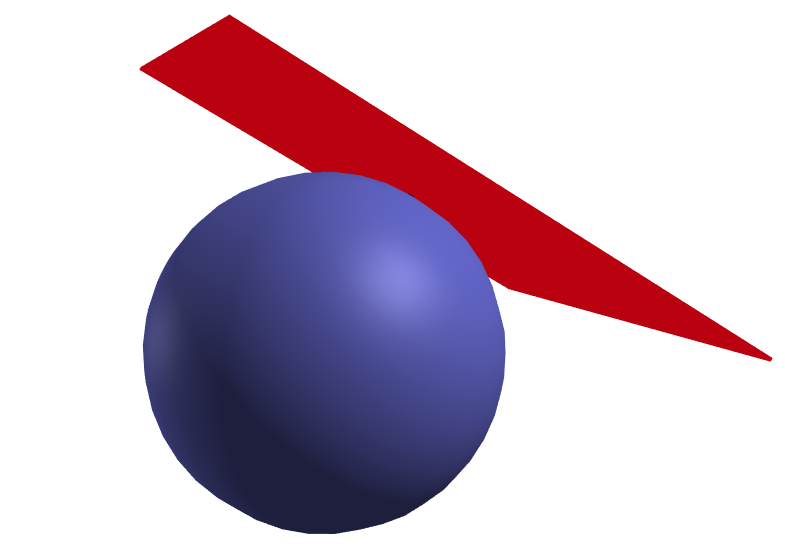
\includegraphics[height=5cm]{figures/tangent_plane.tikz}
        \caption{
            When linearizing about a point $q$ on an sphere $\mathbb{S}^{n-1}$ in 
            n-dimensional space, the tangent space $T$ is a plane living in $\R^{n-1}$, 
            illustrated here with $n=3$. Therefore, when linearizing about a unit 
            quaternion $q \in \Q$, the space of differential rotations lives in $\R^3$.
        }
        \label{fig:tangent_plane}
    \end{figure}
        
        Derivatives consider the effect an infinitesimal perturbation to the input has on
        an infinitesimal perturbation to the output. For vector spaces, the composition
        of the perturbation with the nominal value is simple addition and the
        infinitesimal perturbation lives in the same space as the original vector. For
        unit quaternions, however, neither of these are true; instead, they compose
        according to \eqref{eq:quat_mult}, and infinitesimal unit quaternions are (to
        first order) confined to a 3-dimensional plane tangent to $\Q$ (see Fig.
        \ref{fig:tangent_plane}).

        The fact that differential unit quaternions are three-dimensional should make
        intuitive sense: Rotations are inherently three-dimensional and differential
        rotations should live in the same space as angular velocity, i.e. $\R^3$.
        
        There are many possible three-parameter representations for small rotations in
        the literature. Many authors use the exponential map \cite{Baillieul1978,
        Zefran1998, Lee2008, Saccon2013, Sola2017, Fan2016, watterson2018trajectory},
        while others have used the Cayley map (also known as Rodrigues parameters)
        \cite{Kobilarov2011, Kobilarov2014}, Modified Rodrigues Parameters (MRPs)
        \cite{Terzakis2018}, or the vector part of the quaternion \cite{Fresk2013}.
        We choose Rodrigues parameters \cite{markley2014fundamentals} because they are
        computationally efficient and do not inherit the sign ambiguity associated with
        unit quaternions. The mapping between a vector of Rodrigues parameters $\phi \in
        \R^3$ and a unit quaternion $q$ is known as the Cayley map: \begin{equation}
        \label{eq:cayley}
            q = \varphi(\phi) = \frac{1}{\sqrt{1 + \norm{\phi}^2}} \begin{bmatrix} 1 \\ \phi \end{bmatrix}.
        \end{equation}
        We will also make use of the inverse Cayley map:
        \begin{equation}
            \phi = \varphi^{-1}(q) = \frac{q_v}{q_s}.
        \end{equation}

    \subsection{Jacobian of Vector-Valued Functions}
        When taking derivatives with respect to quaternions, we must take into account
        both the composition rule and the nonlinear mapping between the space of unit
        quaternions and our chosen three-parameter error representation.

        Let $\phi \in \R^3$ be a differential rotation applied to a function with
        quaternion inputs $y = h(q): \Q \to \R^p$, such that
        \begin{equation} \label{eq:vector_function}
            y + \delta y = h(L(q) \varphi(\phi)) \approx h(q) +  \nabla h(q) \phi.
        \end{equation}
        We can calculate the Jacobian $\nabla h(q) \in \R^{p \times 3}$ by
        differentiating \eqref{eq:vector_function} with respect to $\phi$, evaluated at
        $\phi = 0$:
        \begin{equation} \label{eq:quat_gradient}
            \nabla h(q) = \pdv{h}{q} L(q) H := \pdv{h}{q} G(q) 
                        = \pdv{h}{q} \begin{bmatrix} 
                            -q_v^T \\ 
                            sI_3 + \skewmat{q_v}
                        \end{bmatrix}
        \end{equation}
        where $G(q) \in \R^{4 \times 3}$ is the \textit{attitude Jacobian}, which
        essentially becomes a ``conversion factor'' allowing us to apply results from
        standard vector calculus to the space of unit quaternions. This form is
        particularly useful in practice since $\pdv*{h}{q} \in \R^{p \times 4}$ can be
        obtained using finite difference or automatic differentiation.
        As an aside, although we have used Rodrigues parameters, $G(q)$ is actually the
        same (up to a constant scaling factor) for any choice of three-parameter attitude
        representation.

    \subsection{Hessian of Scalar-Valued Functions}
	    If the output of $h$ is a scalar ($p = 1$), then we can find its Hessian by
	    taking the Jacobian of \eqref{eq:quat_gradient} with respect to $\phi$ using the
        product rule, again evaluated at $\phi = 0$:

	    \begin{equation} \label{eq:quat_hessian}
            \nabla^2 h(q) = G(q)^T \pdv[2]{h}{q} G(q) + I_3 \pdv{h}{q}q,
	    \end{equation}
	    where the second term comes from the second derivative of $\varphi(\phi)$.
	    Similar to $G(q)$, this ends up being the same (up to a scaling factor) for any
        choice of three-parameter attitude representation.
        
    \subsection{Jacobian of Quaternion-Valued Functions}
        We now consider the case of a function that maps unit quaternions to unit
        quaternions, $q' = f(q) : \Q \to \Q$. Here we must also consider the non-trivial
        effect of a differential value applied to the output, i.e.:
        \begin{equation} \label{eq:dqoutput}
            L(q') \varphi(\phi') = f(L(q)\varphi(\phi)) .
        \end{equation}
        Solving \eqref{eq:dqoutput} for $\phi'$ we find,
        \begin{equation} \label{eq:phiprime}
            \phi' = \varphi^{-1} \left( L(q')^T f(L(q)\varphi(\phi)) \right) \approx \nabla f(q) \, \phi.
        \end{equation}
        Finally, the desired Jacobian is obtained by taking the derivative of
        \eqref{eq:phiprime} with respect to $\phi$:
        \begin{equation} \label{eq:quat_jacobian}
            \nabla f(q) = H^T L(q')^T \pdv{f}{q} L(q) H = G(q')^T \pdv{f}{q} G(q).
        \end{equation}
        The leading $G(q')^T$ comes from the fact that as $\phi' \to 0$, $L(q') f(q) \to
        I_q$, where $I_q$ is the quaternion identity. Differentiating through the inverse
        map, evaluated at the quaternion identity, we find that $\pdv*{\varphi^{-1}}{q}
        \to H^T$ for any three-parameter attitude representation.


\section{Modifying Newton's Method} \label{sec:Wahbas}

    Newton's method uses derivative information about a function to iteratively
    approximate its roots. For unconstrained systems, this method is highly effective,
    and can exhibit quadratic convergence. For constrained systems, the updated parameter
    can be projected back onto the feasible set at each iteration, but without the same
    convergence guarantees. For the constraints on $SO(3)$, Newton's method struggles to
    converge past a certain threshold due to this projection. By leveraging the
    quaternion calculus introduced, Newton's method can be modified to implicitly account
    for these constraints. To demonstrate this, we will examine Wahba's Problem. In 1965,
    Grace Wahba proposed the criterion for a least squares estimate of a spacecraft's
    attitude from vector measurements \cite{markley2014fundamentals}. We will solve this
    problem using a standard nonlinear least squares method, as well as a method that
    exploits the true group structure of $SO(3)$ using the quaternion calculus presented
    here.
    

    \subsection{Methodology}

    Given known vectors in some inertial frame, ${}^N v_i$, and measurements of these
    vectors in some body fixed frame, ${}^B v_i$, our goal is to determine the relative
    rotation from the body to inertial frame ${}^N q^B$, expressed as a quaternion. We
    can define Wahba's loss function as the following: 
    \begin{align} \label{eq:wahba_loss}
        L &= \sum_i w_i \norm{{}^N v_i - {}^N A(q)^B \,\, ^Bv_i }_2^2. = \norm{r_i(q)}_2^2 
    \end{align} 
    where $r_i(q)$ is the residual vector.

    We can solve for ${}^N q^B$ using a nonlinear least squares method minimizing
    Wahba's loss function:
    \begin{mini*}
        {q}{ \norm{r(q)}_2^2 }{}{}
        \addConstraint { q\in SO(3).}
    \end{mini*}
    
    Following the typical approach for Newton's method, we minimize \eqref{eq:wahba_loss}
    by setting the gradient to zero:
    \begin{equation} \label{eq:newton_foc}
        \begin{aligned}
            \pdv{L}{q}^T &= \sum_i \pdv{r(q)}{q}^T r_i{q} := J^T r(q) = 0 \\
              &= \sum_i (-2 H^T R(q)^T R({}^B \hat{v}_i)^T r(q).
        \end{aligned}
    \end{equation}
    which can be obtained from the chain rule and \eqref{eq:quaternion_rotation}. 

    Treating $q$ as a vector in $\R^4$, we obtain a solution to \eqref{eq:newton_foc}
    using the Moore-Penrose pseudoinverse, $\delta q = (J^T J)^{-1} J^T$, and our
    next candidate quaternion via simple addition, $q_{k+1} = q_k + \delta q$. Since
    $q_{k+1}$ will no longer be unit norm, we project it back on the unit sphere via
    the projection operator $\Pi(q) = q / \norm{q}$. This ``projected'' Newton approach
    is summarized in Algorithm \ref{alg:pgn}.

    \begin{algorithm} 
    	\begin{algorithmic}[1]
    		\caption{Projected Gauss-Newton Method}\label{alg:pgn}
    		\State $k = 0$
    		\While{significant progress}
    		    \State $J = \pdv{r(q_k)}{ \partial q}$ 
    		    \State $ \delta q = -(J^TJ)^{-1}J^T r(q_k)$ 
    		  %  \State $q_{n+1} = \text{normalize}(q_n + q_{step})$ 
    		  \State $q_{k+1} = \Pi_{SO(3)}(q_k + \delta q)$ 
    		    \State $k = k + 1$
    		\EndWhile
    	\end{algorithmic}
    \end{algorithm}
    
    Alternatively, if we instead minimize with respect to a differential quaternion $\phi$,
    we adapt the algorithm by simply ``correcting'' our Jacobian $J$ using 
    \eqref{eq:quat_jacobian}:
    \begin{equation} 
        \bar{J} = \pdv{r(\mathbf{q} \otimes \varphi(\phi))}{\phi} = \pdv{r(q)}{q} G(q).
    \end{equation}
    We obtain our step---this time in the actual tangent space---as before:
    $\phi = (\bar{J}^T \bar{J})^{-1} \bar{J}^T)$. To obtain our next iterate, we ``add'' the
    step using the correct notion of composition for the group: 
    $\q_{k+1} = \q_k \otimes \varphi(\phi)$. This ``multiplicative'' Newton algorithm is 
    summarized in Algorithm \ref{alg:mgn}.

    \begin{algorithm} 
    	\begin{algorithmic}[1]
    		\caption{Multiplicative Gauss-Newton Method}\label{alg:mgn}
    		\State $k = 0$
    		\While{significant progress}
    		    \State $\bar{J} = \pdv{r(q_k)}{q} G(q_k)$ \Comment{quaternion adjusted Jacobian}
    		    \State $ \phi = -(\bar{J}^T \bar{J})^{-1} \bar{J}^T r(q_k)$ 
    		    \State $\q_{k+1} = \q_k \otimes \varphi(\phi)$ \Comment{apply step multiplicatively}
    		    \State $k = k + 1$
    		\EndWhile
    	\end{algorithmic}
    \end{algorithm}



    \subsection{Results}
    As illustrated in Figure \ref{fig:wahba_convergence}, it is clear that by projecting 
    back onto the unit quaternion at each iteration make initial progress, but fails to 
    exhibit the quadratic convergence typical of a Newton method. By optimizing directly 
    in the space of differential quaternions, we achieve the expected quadratic convergence.
    It should also be clear from the previous section that the adaptations to the original
    Newton method are simple and straightforward, highlighting both the effectiveness and
    value of the proposed approach.
    \begin{figure}

        \centering
        \includegraphics[width=\columnwidth, height=5cm]{figures/wahba_convergence.tikz}
        \caption{Convergence comparison for Wahba's problem. By performing Newton's method
        on the error quaternion and applying the result to the full quaternion we achieve
        quadratic convergence, whereas the more na\"ive approach doesn't converge to zero
        error. The angle error is calculated relative to the true analytical solution obtained
        via an SVD decomposition.}
        \label{fig:wahba_convergence}
    \end{figure}
    % \begin{figure}[H]
    %     \centering
    %     \includegraphics[width=\columnwidth, height=5cm]{figures/kevins_plots/convergence_plot.tikz}
    %     \caption{Convergence comparison for Wahba's problem. By performing Newton's method
    %     on the error quaternion and applying the result to the full quaternion we achieve
    %     quadratic convergence, whereas the more na\"ive approach doesn't converge to zero
    %     error.}
    %     \label{fig:wahba_convergence}
    % \end{figure}

\section{Trajectory Optimization on $\R^n \times SO(3)$} \label{sec:trajopt}
    Here we outline the modifications to the ALTRO solver \cite{howell2019altro}, to
    solve trajectory optimization problems for rigid bodies, which extends easily to
    arbitrary systems in $\R^n \times SO(3)$. ALTRO is an efficient solver for constrained
    nonlinear optimization problems that uses iterative LQR (iLQR) with an augmented
    Lagrangian framework.

    We consider a trajectory optimization problem of the form:
    \begin{mini}[2]
        {x_{0:N},u_{0:N-1}}{\ell_f(x_N) + \sum_{k=0}^{N-1} \ell(x_k,u_k) }{}{}
        \addConstraint{x_{k+1} = f(x_k,u_k)}
        \addConstraint{g_k(x_k,u_k)}{\leq 0}
        \addConstraint{h_k(x_k,u_k)}{=0}
        \label{discrete_trajopt},
    \end{mini}
    where $x$ and $u$ are the state and control vectors as described in Sec. \ref{sec:rigidbody_dynamics},
    $f$ are the dynamics as defined in \eqref{eq:rigid_body_dynamics}, $\ell$ is a general
    nonlinear cost function,
    $N$ is the number of time steps, and $g_k$, $h_k$ are general nonlinear inequality and 
    equality constraints.

    Like most gradient or Newton-based methods for optimization, ALTRO approximates the 
    nonlinear functions $f, \ell, g,$ and $h$ with their first or second-order Taylor series
    expansions. Leveraging the methods from Sec: \ref{sec:Quaternion_Calculus}, we adapt the
    algorithm to optimize directly on the error state $\delta x \in \R^{12}$. 

    We begin by linearizing the dynamics about the reference trajectory using
    \eqref{eq:quat_jacobian}. Our linearized error dynamics become
    \begin{equation} \label{eq:linearized_dynamics}
        \delta x_{k+1} = A_k \delta x_k + B_k \delta u_k 
    \end{equation}
    where \begin{equation}
        \begin{aligned}
            A_k = E(\bar{x}_{k+1})^T \pdv{f}{x}|_{\bar{x}_k,\bar{u}_k} E(\bar{x}_k), \\
            B_k = E(\bar{x}_{k+1})^T \pdv{f}{u}|_{\bar{x}_k,\bar{u}_k},
        \end{aligned}
    \end{equation}
    and $\delta x_k \in \R^{12}$ and $E(x_k) \in \R^{12 \times 13}$ are the state error and state error Jacobian:
    \begin{equation} \label{eq:state_error}
        \setlength\arraycolsep{1pt}
        \delta x_k = \begin{bmatrix} 
            r_k - \bar{r}_k \\ \varphi^{-1}(\bar{\q}_k^{-1} \otimes \q_k) \\ v_k - \bar{v}_k \\ \omega_k - \bar{\omega}_k 
        \end{bmatrix}\!, \;
        E(x) = \begin{bmatrix}
            I_3 & & & \\
            & G(q) & & \\
            & & I_3 & \\
            & & & I_3 \\
        \end{bmatrix}\!.
    \end{equation}
    
    By applying \eqref{eq:quat_gradient} and \eqref{eq:quat_hessian} to our nonlinear cost
    functions $\ell$ and 
    \eqref{eq:quat_jacobian} to the nonlinear constraint functions $g_k$ and $h_k$, we can calculate
    the second-order expansion 
    \begin{multline}
        \delta \ell(x,u) \approx  \half \delta x^T \ell_xx \delta x
            + \half \delta u^T \ell_{uu} \delta u + \delta_u^T \ell_{ux} \delta u \\
            + \ell_x^T \delta x^T + \ell_u^T \delta u 
    \end{multline}
    of the augmented Lagrangian cost function:
    \begin{equation}
        \mathcal{L}_A = \mathcal{L}_N(x_N,\lambda_N,\mu_N) + 
            \sum_{k=0}^{N-1} \mathcal{L}_k(x_k,u_k,\lambda_k,\mu_k)
    \end{equation}
    where
    \begin{equation}
        \mathcal{L}_k(x,u,\lambda,\mu) = \ell(x,u) + 
            (\lambda + \half I_\mu c(x,u))^T c(x,u),
    \end{equation}
    with $c(x,u)$ being the concatenation of the constraints $f,g$, and $h$ at a given time step,
    and $I_\mu$ the penalty matrix.

    With this expansion, we calculate the expansion of the ``action-value function'' $Q(x,u)$
    as normal:
    \begin{align}
        Q_{xx} &= \ell_{xx} + A_{k}^T P_{k+1} A_{k} \label{Qxx_exp}\\
        Q_{uu} &= \ell_{uu} + B_{k}^T P_{k+1} B_{k} \label{Quu_exp}\\
        Q_{ux} &= \ell_{ux} + B_{k}^T P_{k+1} A_{k} \label{Qux_exp}\\
        Q_x &= \ell_x  + A_{k}^T p_{k+1} \label{Qx_exp}\\
        Q_u &= \ell_u + B_{k}^T p_{k+1} \label{Qu_exp},
    \end{align}
    from which we can calculate the quadratic expansion of the cost-to-go 
    $P_k \in \R^{12 \times 12}$, $p_k \in \R^{12}$, and optimal linearized feedback gains 
    $K_k \in \R^{m \times 12}$ and $d_k \in \R^m$ by starting at the terminal state and
    resursing backward in time along the trajectory during the ``backward pass'' of the iLQR
    algorithm. During the ``forward pass'', the dynamics are simulated forward in time using
    the feedback gains computed during the backward pass. At each time step, the control is 
    calculated using the linear feedback controller: 
    \begin{equation} \label{eq:mlqr_control}
        u_k = K_k \delta x_k + \bar{u}_k.
    \end{equation}
    where $\bar{u}_k$ is the control value from the previous iteration, and $\delta x$ is
    computed using \eqref{eq:state_error}, with $x_k$ being the current state estimate
    and $\bar{x}_k$ the state from the previous iteration. The rest of the algorithm is
    left unchanged. For more details on the ALTRO algorithm, the reader is encouraged to
    refer to the original paper \cite{howell2019altro}.

    \subsection{Quaternion Cost Functions} \label{sec:cost_functions}
        In addition to the straight-forward modifications to the ALTRO algorithm itself, we
        need to carefully consider the types of cost functions we minimize. We frequently
        minimize costs that penalize distance from a goal state, e.g. $\half (x-x_g)^T Q
        (x-x_g)$; however, na\"ive substraction of unit quaternions is ill-defined. We
        propose two different cost functions that accomplish similar behavior.
        For sake of clarity and space, we only consider the costs on the quaternion
        variables: costs on the other states and the control variables remain unaffected.
        
        \subsubsection{Error Quadratic} \label{sec:error_quadratic}
            Rather than simple subtraction, we can use a quadratic function on the
            three-parameter error state \eqref{eq:state_error}:
            \begin{equation} \label{eq:error_quadratic}
                J_\text{err} = \half \phi^T Q \phi 
                = \half \left(\varphi^{-1}(\delta q)\right)^T Q 
                        \left(\varphi^{-1}(\delta q)\right).
            \end{equation}
            where $\delta q = L(q_g)^T q$, and $\phi = \varphi{\delta q}$. The gradient
            and Hessian of \eqref{eq:error_quadratic} are
            \begin{equation}
                \nabla J_\text{err }= \phi^T Q  D(\delta q)  G(\delta q)
            \end{equation}
            \begin{multline}
                \nabla^2 J_\text{err} = 
                    G(\delta q)^T \! \left(
                    D(\delta q)^T Q D(\delta q) + \nabla D \right) G(\delta q)  \\
                    + I_3 (\phi^T Q  D(\delta q)) \delta q %\\
            \end{multline}
            where, for the Cayley map,
            \begin{equation}
                D(q) = \pdv{\varphi^{-1}}{q} = -\frac{1}{q_s^2}\begin{bmatrix}
                    q_v \;\; & -\frac{1}{q_s} I_3
                \end{bmatrix}
            \end{equation}
            \begin{equation}
                \nabla D = \pdv{q}(D(q)^T Q \phi) 
                = -\frac{1}{q_s^2} \begin{bmatrix} 
                    -2 \frac{q_v}{q_s}^T Q \phi & \phi^T Q \\
                                   Q \phi & 0 \\
                \end{bmatrix}.
            \end{equation}

        \subsubsection{Geodesic Distance} \label{sec:geodesic}
            Alternatively, we can use the geodesic distance between two quaternions
            \cite{Kuffner2004},
            \begin{equation} \label{eq:quat_geodesic}
                J_\text{geo} = (1-\abs{q_g^T q}) ,
            \end{equation}
            whose gradient and Hessian are,
            \begin{align}
                \nabla J_\text{geo} &= \pm q_g^T G(q) \\
                \nabla^2 J_\text{geo} &= \pm I_3 q_g^T q ,
            \end{align}
            where the sign of the Hessian corresponds to the sign of $q_d^T q$.


\section{Experiments} \label{sec:experiments}
    In this section we present several trajectory optimization problems for systems that
    undergo large changes in attitude: an airplane barrell roll, a quadrotor flip, and a
    satellite with flexible modes that must slew to a new orientation while avoiding a 
    ``keep out'' orientation zone. All results were run on a desktop computer with an 
    AMD Ryzen 2950x processor with 40 GB of RAM. 
    All problems are run using ALTRO, first without any of the modifications presented 
    in the current paper, labeled ``original'', and then using the modifications listed
    in Sec. \ref{sec:trajopt} and the geodesic cost funtion described in Sec. \ref{sec:geodesic},
    labeled ``modified''.
    Timing results are summarized in Table \ref{tab:timing_results}.
    All experiments were solved to a constraint satisfaction tolerance of $10^{-5}$ and 
    discretized with a 4th order Runge-Kutta integrator.
    Code for all experiments is available on 
    \href{https://github.com/RoboticExplorationLab/PlanningWithAttitude}
    {GitHub\footnote{\url{https://github.com/RoboticExplorationLab/PlanningWithAttitude}}}.

    \begin{table}
        \centering
        \begin{tabular}{lll}
\toprule 
Problem & Iterations & time (ms) \\
\midrule 
barrellroll & 47 / 36 & 94.54 / 78.65 \\
quadflip & 58 / 28 & 457.58 / 217.69 \\
satellite & 35 / 35 & 446.52 / 517.47 \\
\bottomrule 
\end{tabular}

        \label{tab:timing_results}
        \caption{Trajectory Optimization Timing Results}
    \end{table}
        
    \subsection{Satellite Attitude Keep-Out}
    A spacecraft with flexible appendages must perform a 150 degree slew, while ensuring
    that a star tracker line-of-sight does not cross within 40 degrees of the sun. The
    attitudes that result in the star tracker pointing too close to the sun will be
    referred to as a keep-out zone. The flexible body spacecraft dynamics are based on
    the truncated hybrid coordinate model, with the three largest modes captured
    \cite{Tracy2020}. We can guarantee the star tracker body fixed vector ($^Br_{st}$)
    does not look within 40 degrees of the inertial sun vector ($^Nr_{sun}$) by
    formulating the following constraint:
    \begin{equation}
        \langle ^N q ^B {}^Br_{st} , ^Nr_{sun}\rangle \leq \cos(40 ^\circ).
    \end{equation}
    Due to this constraint on the feasible attitudes, an eigen-axis slew trajectory
    planner may end up violating this keep-out zone \cite{markley2014fundamentals}. ALTRO
    can generate a feasible trajectory for this problem since it is able to reason about
    the nonlinear flexible spacecraft dynamics, actuator constraints, and the star
    tracker line of sight constraint.
        \begin{figure}
            \centering
            \includegraphics{figures/kevins_plots/attitude_slew_plot.tikz}
            \caption{Visualization of the flexible spacecraft slew with a dedicated keep-out zone. Attitude is parameterized with a Rodrigues parameter to visualize the trajectory in three dimensions. The constraint surface represents attitudes where the star tracker line-of-sight is within 40$^\circ$ of the sun. The unconstrained solution violates this constraint, while the constrained solution is able to avoid the keep out zone.}
        \end{figure}


    \subsection{Airplane Barrel Roll}

        An airplane model with aerodynamic coefficients fit from real wind-tunnel data is
        tasked to do a barrel roll by setting a high terminal cost for being upside-down,
        see Fig. \ref{fig:barrellroll}. The solver is initialized with level flight trim
        conditions. The convergence of the different versions is compared in Fig.
        \ref{fig:c_max_convergence}. For both the quadrotor flip and the airplane barrel
        roll, the modified version of ALTRO converged faster than original version.
        For these highly aerobatic maneuvers, we achieve, as expected, better
        performance by correctly leveraging the structure of the rotation group during
        the optimization routine.

        We also compared the ``error quadratic'' cost function described in Section
        \ref{sec:error_quadratic} to the geodesic cost function in Section
        \ref{sec:geodesic}. The geodesic cost was more efficient, both in term of
        iterations and computation time, taking only 36 iterations and 1.8 ms/iteration
        vs 76 iterations and 7.6 ms/iteration for the error quadratic. Not only is the
        geodesic cost function much cheaper to compute, it also converges much faster
        than the geodesic cost function. This could be due to the strong nonlinearities
        introduced when computing the quaternion error, making it more difficult to
        optimize.
        
        \begin{figure}[h]
            \centering
            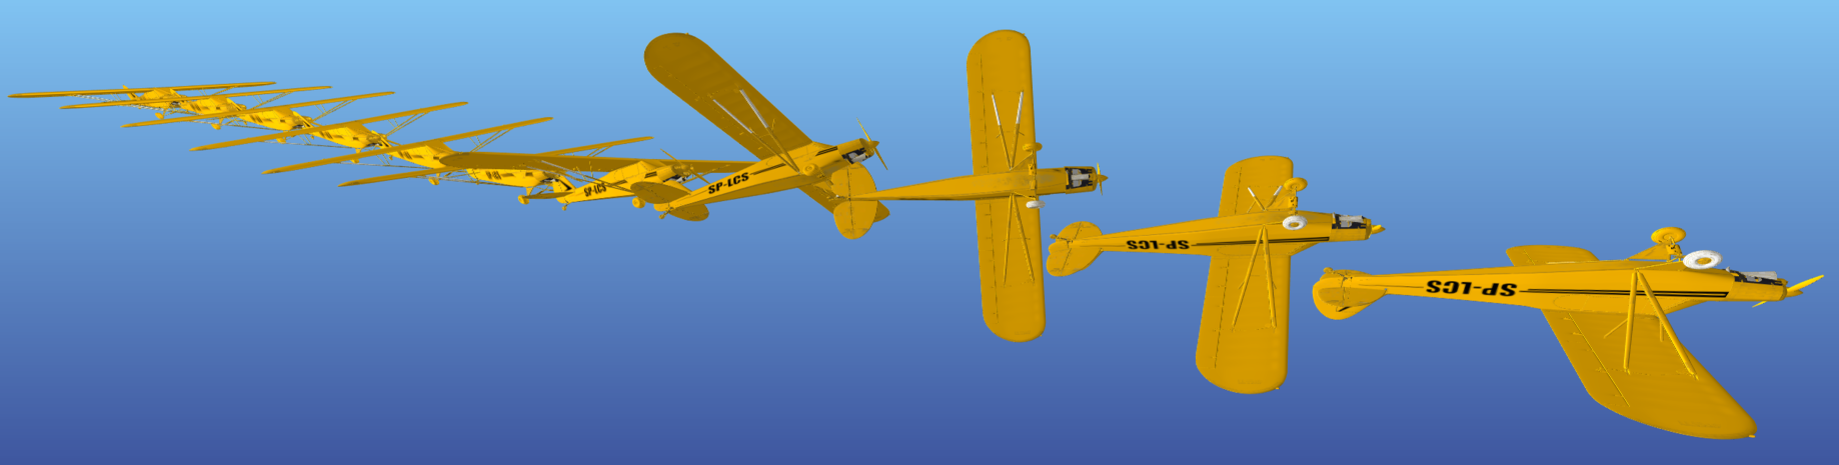
\includegraphics[width=\columnwidth]{figures/barrellroll.png}
            \caption{Barrel roll trajectory computed by iterative MLQR using a terminal cost to encourage an upside-down attitude.}
            \label{fig:barrellroll}
        \end{figure}

        \begin{figure}[h]
            \centering
            \includegraphics[height=4cm,width=\columnwidth]{figures/c_max_convergence.tikz}
            \caption{Constraint convergence when solving the barrel roll problem. Compares 
            the convergence of the original version of ALTRO versus the new, modified version
            that optimizing on the error state.}
            \label{fig:c_max_convergence}
        \end{figure}

    \subsection{Quadrotor Flip}
        We sucessfully optimized a 360 degree flip trajectory for a quadrotor using the 
        modified version of ALTRO.
	    Four intermediary knotpoints were used to encourage the quadrotor to be at angles
        of \ang{90}, \ang{180}, \ang{270}, and \ang{360} around an approximately circular arc.
        The quadrotor was constrained
	    to stay above the floor and move to a goal state 2 meters away in the $+y$
	    direction. The solver was initialized with a dynamically infeasible trajectory
	    that linearly interpolates between the initial and final states, rotating the
        quad around the x-axis a full \ang{360}.

	    Figure \ref{fig:quad_flip} shows snapshots of the trajectory as generated using
	    ALTRO. The original version of ALTRO, even after significant tuning efforts,
	    would not converge to the desired solution. It instead got halfway and then
	    ``unwound'' 360 degrees and then continued rotating to the final orientation.
	    This behavior is common and expected when attempting optimization that does not
	    properly account for the group structure of rotations. It is also worth noting
	    that this problem could not be solved using any three-parameter attitude
	    representation, since it passes through the singularities at $90\degree,
	    180\degree$, and $360\degree$ for Euler angles, Rodrigues parameters, and
	    Modified Rodrigues Parameters, respectively.

        \begin{figure}[t]
            \centering
            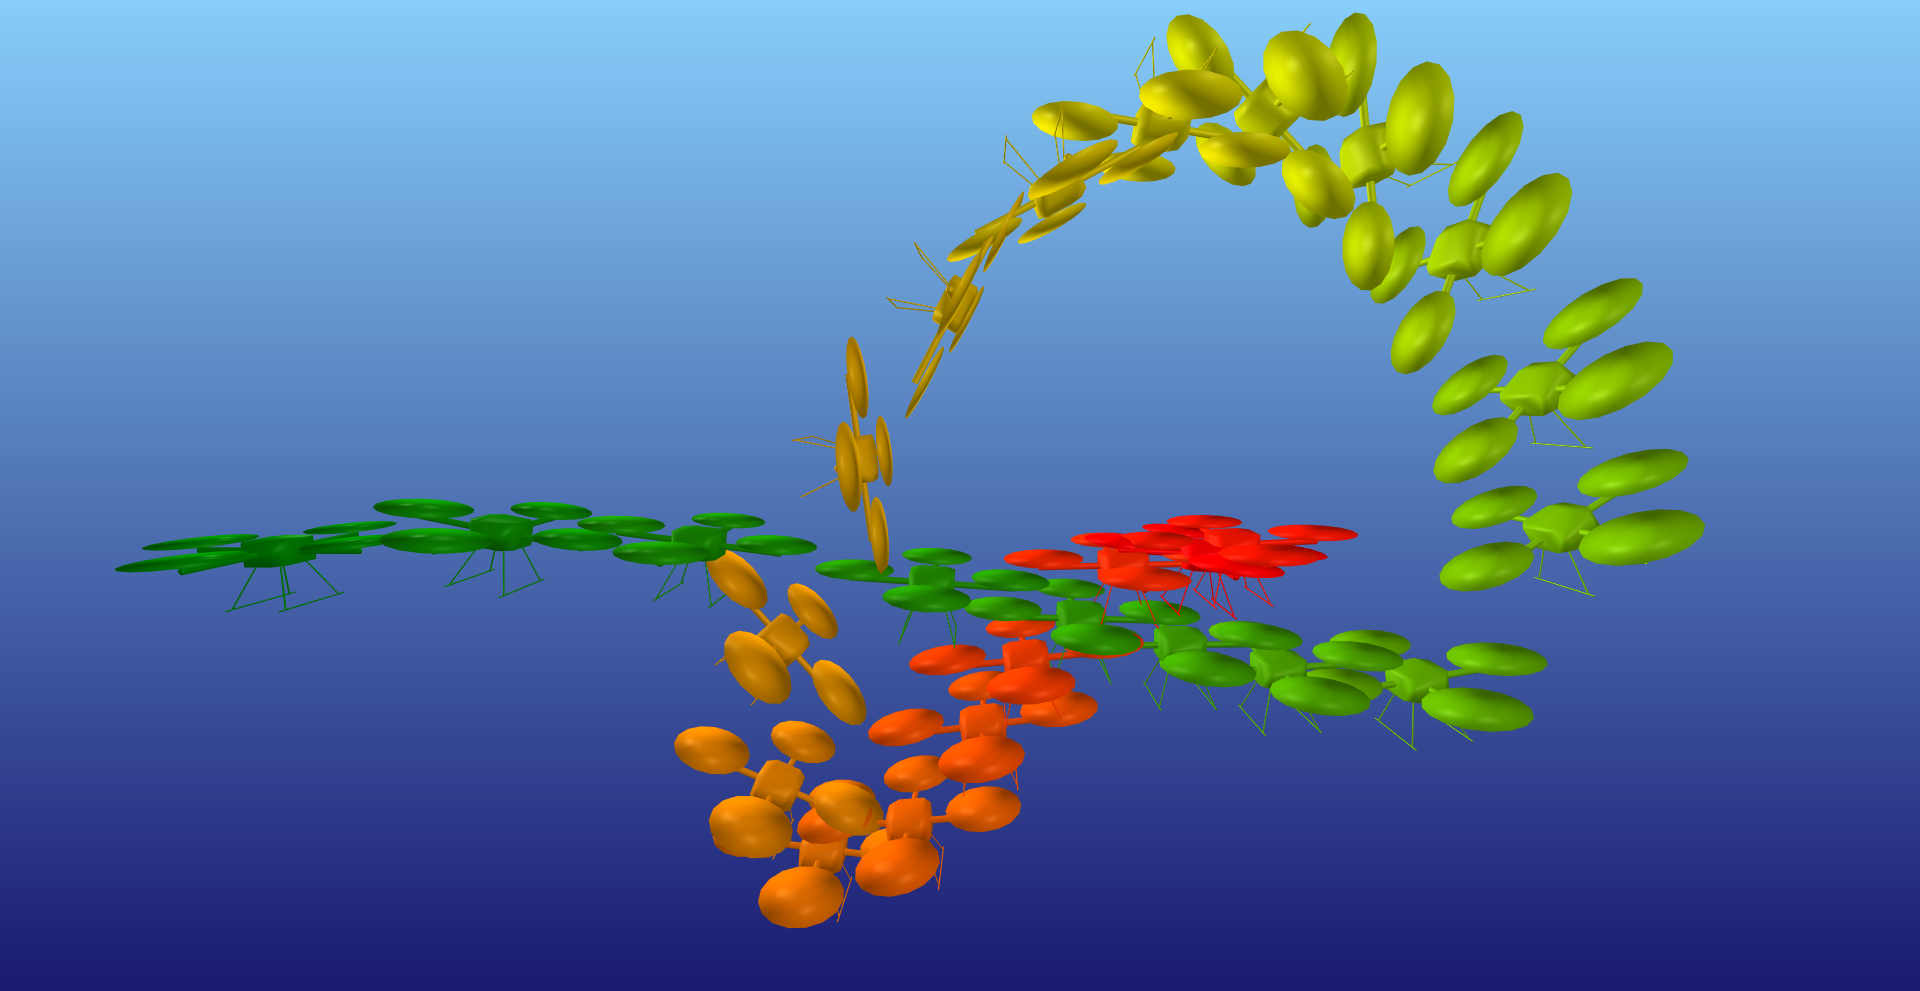
\includegraphics[width=\columnwidth]{figures/quadflip.png}
            \caption{Snapshots of the quadrotor flip trajectory. The
                gree-colored quadrotors represent the state near t=0 s and the
                red-colored quadrotors represent the state near t=5.0 s
            }
            \label{fig:quad_flip}
        \end{figure}    
    

\section{Conclusions} \label{sec:conclusion}
    We have presented a general, unified method for planning and control on rigid-body
    systems with arbitrary attitude using standard linear algebra and vector calculus.
    We have demonstrated that the application of this methodology is straightforward and
    yields substantion improvements in the convergence of Newton-based methods (see Fig. 
    \ref{fig:wahba_convergence}) while also offering improvements for nonlinear constrained
    trajectory optimization for floating-base systems (see Table \ref{tab:timing_results}).
    
    With the modifications presented, ALTRO can solve problems few other methods for 
    trajectory optimization can. Many state-of-the-art methods such as direct 
    collocation or sequential convex programming rely on commercial, proprietary, or 
    general-purpose solvers whose internal numerics often are abstracted away from the user. 
    By exploiting both the unique Markovian structure of the trajectory optimization problem
    and the group structure of rotations, ALTRO will likely be able to solve new classes of 
    problems with at or near real-time performance. Future work will focus on continued 
    refinement of the implementation and benchmarking against current state-of-the-art 
    methods for trajectory optimization and other specialized solvers for optimization on
    manifolds.

    Additionally, the methods presented here can easily be leveraged to adapt other classes
    of gradient or Newton-based algorithms to exploit the structure of 3D rotations. Future
    work may include adaptation of methods for state estimation, localization, design, or 
    other methods for motion planning such as direct collocation. 
    
    Future work will also include the application of these methods to multi-body robotic
    systems, such as humanoids or quadrupeds, especially in methods that exploit 
    ``maximal'' coordinates that include the 3D orientation of each body \cite{brudigam2020linear}. 

\paragraph*{Acknowledgements}
This material is based upon work supported by the National Science Foundation Graduate
Research Fellowship Program under Grant No. DGE-1656518. Any opinions, findings, and
conclusions or recommendations expressed in this material are those of the author(s) and
do not necessarily reflect the views of the National Science Foundation


\printbibliography

\end{document}